%\vspace*{-20mm}
			\section{Significato di relazione}

																				\epigrafe{\emph{Solitamente mi ci vogliono tre settimane
																								per preparare un valido discorso improvvisato}.}
																					{Mark Twain}



\capolettera[4]{C}{he cos'è esattamente} una relazione? In prima approssimazione è possibile dire che una relazione è un particolare testo di tipo \hlightit{argomentativo} e \hlightit{informativo}. È argomentativo perché ha lo scopo di sostenere una tesi su basi logico-scientifiche (saggi, report, analisi, tesi accademiche, articoli \ecc), è informativo perché arricchisce le conoscenze del lettore su un determinato argomento.

L'unione delle proprietà di un testo argomentativo e di uno informativo danno luogo a quello che prende il nome di \hlightit{testo espositivo}, tipologia di documento di cui fanno parte anche le relazioni tecnico-scientifiche.

La struttura di un testo espositivo --la relazione-- è facilmente riconoscibile per la modalità gerarchica e cronologica con cui vengono organizzate le informazioni. Per facilitare non solo la lettura ma anche la ricerca dei singoli elementi, la relazione è solitamente suddivisa in sezioni dove viene esposta:
%%
\begin{itemize}
 \item la presentazione del problema, ovvero l'oggetto di studio, che essendo semplicemente informativa, costituisce la premessa;
 %%
 \item la tesi che ci si accinge a dimostrare o l'esperimento o la prova eseguita, ovvero lo scopo;
 %%
 \item gli argomenti a sostegno della tesi o le teorie e le ipotesi che sono alla base dell'esperimento o della prova;
 %%
 \item eventuali antitesi da confutare o altri metodi utilizzati in passato anche da altri;
 %%
 \item eventuali argomenti a sfavore dell'antitesi o dei metodi già utilizzati per condurre il medesimo esperimento o prova; 
 %%
 \item esposizione della teoria, delle ipotesi e dei metodi (compresi gli strumenti) utilizzati per raccogliere i dati;
 %%
 \item metodi di calcolo, formule utilizzate e formalizzazione degli errori;
 %%
 \item analisi dei dati e calcoli;
 %%
 \item inserimento delle informazioni ritenute rilevanti in tabelle e grafici. Se ritenuto opportuno, tale informazioni possono essere correlate o completate con altre provenienti da altri studi;
 %%
 \item osservazioni;
 %%
 \item deduzioni, dimostrazioni e conclusioni.
\end{itemize}

Un testo espositivo di questo genere è noto come \hlightit{top-down} perché adotta una logica modulare, perché rende i materiale facilmente disponibile e raggiungibile e perché, chi legge, può immediatamente capire quali parti seguire, trascurare o approfondire.

Il testo espositivo e in particolare la relazione tecnico-scientifica,, deve offrire a chi legge la possibilità di ripetere l'esperimento (la prova \ecc) in modo da ottenere risultati con cui confermare, o eventualmente confutare, le osservazioni e deduzioni fatte dall'autore o dagli autori.

In virtù di ciò, una relazione deve necessariamente possedere un tono distaccato, impersonale e adottare uno specifico e appropriato registro linguistico con cui eliminare ogni ambiguità.

L'uso di forme personali, di punti di vista, di retorica o di una comunicazione di tipo emotiva, deve essere assolutamente evitata come vanno evitati tutti i grafemi comunicativi non testuali, con cui trasmettere sensazioni e non informazioni oggettive (per esempio puntini di sospensione, punti esclamativi e interrogativi, gli ``\textit{eccetera}''). Una relazione deve quindi essere chiara, completa, oggettiva, coerente e organizzare adeguatamente fatti e informazioni. Si adotterà quindi:
%%
\begin{itemize}
 \item un preciso lessico conforme alla natura del documento che ci si accinge a scrivere (ricorrendo, se necessario, anche all'uso di acronimi);
 %%
 \item l'uso di forme impersonali al presente (``\textit{si osserva}'', ``\textit{si prende}'' \ecc) anche in forma passiva (``\textit{è stato fatto}'', ``\textit{è stato misurato}'' \ecc).
\end{itemize}



					\subsection{Uso di termini e parole straniere}

Nel testo in italiano le parole straniere non si declinano al plurale. Per esempio \textbf{non} ``\textit{computers}'' ma ``\textit{computer}''. Il genere delle parole straniere non muta rispetto alla lingua di origine. Si scriverà quindi: ``\textit{l par condicio}'', ``\textit{la Bundesbank}''.

Per le lingue che hanno il genere neutro (tedesco, russo, \ecc) i nomi neutri in italiano si declinano al maschile (per esempio ``\textit{il leitmotiv}''. In inglese, persone e animali nella nostra lingua mantengono il genere di origine, mentre quello delle cose si accordo con quello della corrispondente lingua italiana:
%%
\begin{center}
\textit{la e-mail, il flash, l'information technology, la motherboard}
\end{center}
%%



					\section{Alcune note di carattere tipografico}
					
La tecnologia, la concorrenza e la costante diminuzione dei prezzi, ha reso praticamente accessibile a tutti l'uso di dispositivi mobili, portatili e fissi con cui eseguire programmi, anche non esattamente installati sul proprio dispositivo%%
%%
			\footnote{Come per esempio \hlightit{Google Documents}, un'alternativa cloud e free al pacchetto Office di Microsoft.}
%%
per l'elaborazione di testi, analisi dei dati e la loro memorizzazione su data base.

Gli elaboratori di testo, più noti come \hlightit{word processor}, hanno goduto sin da subito di un'ottima accoglienza da parte di chi, per professione o studio, era costretto a redigere i propri elaborati o a mano o con una vecchia e rumorosa macchina da scrivere.

Con il tempo non solo le loro interfacce sono diventate sempre più \hlightit{user friendly}, ma gli strumenti messi a disposizione sono aumentati e diventati sempre più potenti. L'autore, seppure in teoria, non solo è diventato dattilografo di se stesso, ma si è anche evoluto in un Gutenberg dei nostri tempi.

Si tratta però pur sempre di strumenti, e in quanto tali il loro uso presuppone una conoscenza almeno basilare di ciò che possono offrire. Nelle sezioni che seguono, vengono definite alcuni degli elementi che concorrono per scrivere una relazione tipograficamente accettabile.

Nel caso in cui per scelta o necessità si preferisca scrivere a mano, le indicazioni date continueranno a mantenere la loro validità, con la raccomandazione accessoria di utilizzare una grafia assolutamente leggibile.


								\subsection{Uso dei caratteri di stampa}
								
Le famiglie secondo cui sono organizzati i caratteri di stampa, hanno caratteristiche grafiche e fisiche tali da renderle diverse le une dalle altre. In particolare:
%%
\begin{description}
 \item[stile]: definisce la proprietà grafica del carattere, ovvero il nome (\hlightit{Times}, \hlightit{Helvetica}, \hlightit{Garamound}, \hlightit{Arial}, \ecc);
 %%
 \item[variante]: indica la versione dei caratteri in un determinato \hlightit{stile} (\textbf{bold-grassetto}, \hlightit{italic-corsivo}, \textsc{maiuscoletto}, \ecc);
 %%
 \item[corpo]: indica la dimensione del carattere di stampa misurata in \hlightit{punti tipografici} (``pt'');
 %%
 \item[font]: indica l'insieme dei caratteri con un certo stile grafico e un determinato corpo.
\end{description}


						\subsubsection{Uso delle varianti di un font}
						
Il \hlightit{corsivo} (\hlightit{italic}) viene utilizzato per evidenziare parole, termini, frasi o definizioni. I termini tecnici o specialistici (in taluni casi anche quelli stranieri) possono essere scritti in corsivo la prima volta che compaiono nel testo, mentre nel seguito verranno generalmente scritti in tondo.

il \textbf{grassetto} (\textbf{bold}) viene normalmente utilizzato per la composizione dei titoli dei capitoli, delle sezioni, eccetera. In rari casi può essere utilizzato nel corpo del testo in modo da evidenziare maggiormente un termine ma mai una intera frase.



						\subsubsection{Impaginazione del testo}
						
Per \hlightit{impaginazione} si intende l'armonica e bilanciata disposizione degli elementi di un testo in una o più pagine. In una relazione si raccomanda quindi:
%%
\begin{itemize}
 \item per rendere più scorrevole la lettura ed evitare l'affaticamento della vista, il testo deve essere \hlightit{giustificato}. Tutte le righe di testo dovranno quindi essere allineate fra loro sia a sinistra sia a destra. Nel caso di inizio paragrafo la riga iniziale può lievemente rientrare a destra. Non utilizzare l'allineamento a bandiera (a sinistra);
 %%
 \item la scelta dei margini, ovvero la distanza del testo dai margini destro, sinistro, alto e basso, dipende dal tipo di \hlightit{rilegatura}%%
 %%
				\footnote{Per \hlightit{rilegatura} si intende quella particolare operazione con cui si realizza l'unione delle pagine di un documento, articolo, libro, eccetera. La rilegatura più semplice e rapida è quella che consiste nello \hlightit{spillare} con una spillatrice le pagine. Altri modi rapidi con cui unire le pagine di un documento sono l'uso di \hlightit{dorsetti} di plastica, rilegatrici termiche, a spirale eccetera.}
 %%
 come anche dal corpo del carattere utilizzato per scrivere il documento (tipicamente si sceglie un corpo di $12$pt). In genere si lasciano almeno $25\mm$ in alto e in basso e almeno $20\mm$ a destra e a sinistra della pagina (in alcuni documenti, per esempio quelli notarili, si usano margini anche maggiori);
 %%
 \item Il numero di caratteri per riga deve essere contenuto entro gli $85$ caratteri. Sono valori ottimali quelli compresi tra $80--85$ caratteri (vedi anche fig.~\ref{fig:cei11-17} a pag.~\pageref{fig:cei11-17}). Numeri inferiori sono utilizzati in altri ambiti e in altri tipi di testo%%
				\footnote{Per esempio Robert Bringhurst nel suo \hlightit{The Elements of Typographic Style} considera perfetti $66$ caratteri per riga.}.
 %%
 Il corpo del font deve quindi essere scelto in modo tale che una volta stabiliti i margini il numero dei caratteri per riga siano limitati a $85$;
 %%
 \item ciascun paragrafo deve essere spaziato verticalmente dal precedente in modo da migliorare la leggibilità. Un paragrafo deve essere composto da almeno due o più frasi in modo da analizzare compiutamente un determinato problema o argomento;
 %%
 \item un testo, specie se lungo, deve essere diviso in parti logiche. La suddivisione in capitoli è opportuna, anzi irrinunciabile, per i documenti composti da cinquanta o più pagine. Per i documenti più brevi si raccomanda invece la suddivisione in sezioni in modo da migliorare la ricerca di specifici argomenti. Il titolo della sezione (o del capitolo) viene composto con un corpo carattere più grande di quello utilizzato per il testo. È buona norma riportare il titolo delle sezioni in un indice introduttivo in cui viene specificato anche il numero della pagina in cui inizia;
 %%
 \item l'\hlightit{interlinea}, ovvero lo spazio che separa verticalmente due righe contigue, deve essere singola, al massimo impostata a $1,5$ righe e mai \hlightit{doppia}. 
\end{itemize}
%%
\begin{figure}[htb!]
\centering
    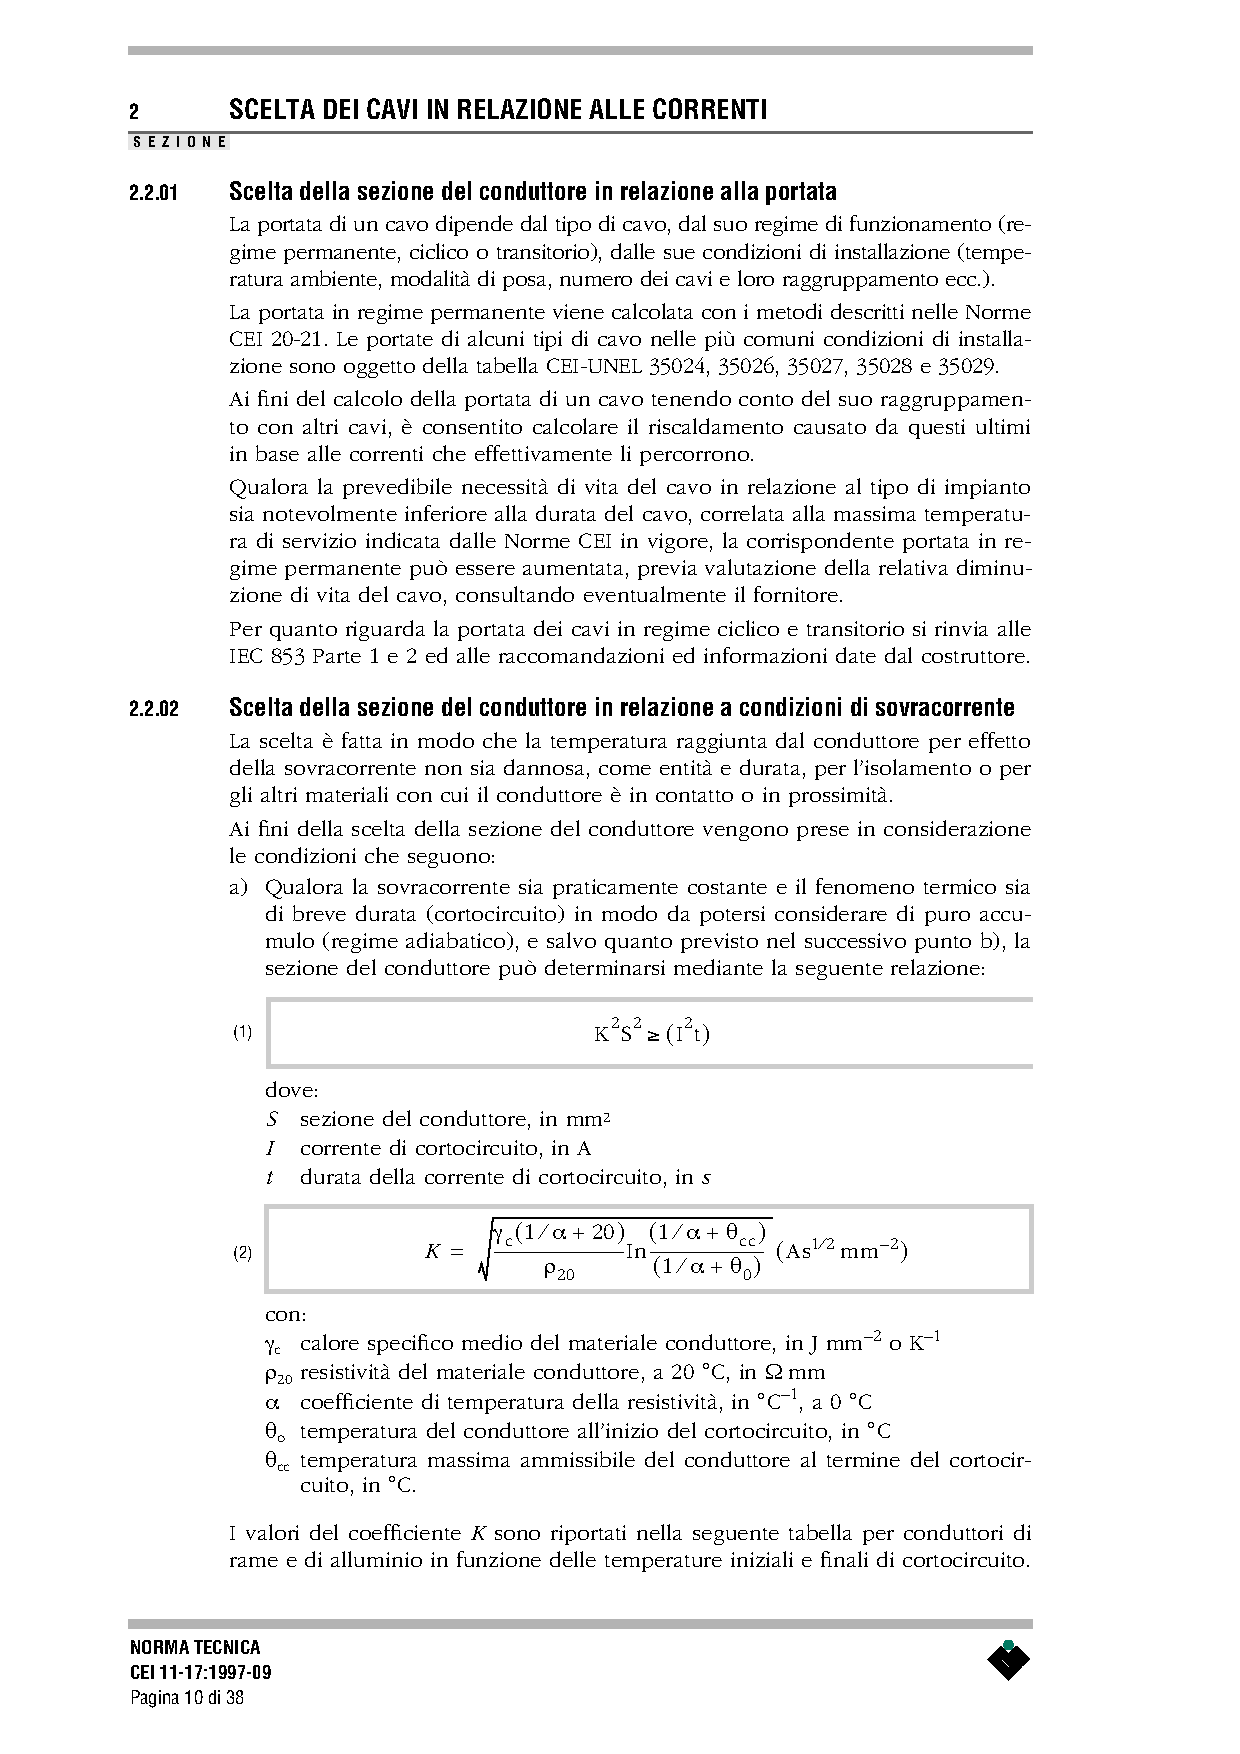
\includegraphics[width=0.86\textwidth]{figure/cei_11-17.pdf}%
    \caption[Pagina di esempio della Norma CEI 11-17.]{Pagina della Norma CEI 11-17. si noti l'ampiezza dei margini e il numero dei caratteri per riga.}
    \label{fig:cei11-17}
\end{figure}


						\section{Le formule}

Le relazioni a contenuto tecnico-scientifico analizzano dati (l'informazione grezza) che vengono utilizzati come termini di specifiche equazioni e formule. La \hlightit{sintassi} e la \hlightit{grammatica} con cui equazioni e formule vengono scritte usa, naturalmente, regole matematiche che si ritengono note e apprese.

Nei casi in cui il documento venga scritto con un word processor, si ritiene tassativo l'uso dell'\hlightit{equation editor} per scrivere formule ed equazioni come anche i calcoli eseguiti.

Le formule devono essere perfettamente leggibili e scritte, tranne alcuni casi, in righe separate. Se il numero delle formule inizia ad essere importante, è buona norma inserire verso il margine destro della stessa riga in cui compaiono, un'etichetta (detta anche \hlightit{label}) numerica. In una qualunque parte del testo ci si potrà così riferire a una specifica formula, utilizzando espressioni come ``\textit{\ldots~la formula~(\ref{eq:ohm}) a pag.\pageref{eq:ohm}~\ldots}''. Per esempio:
%%
\begin{equation}
 R = \frac{V}{I}\label{eq:ohm}
\end{equation}
%%

Nel caso di equazioni fratte, il simbolo che ne determina la relazione (di uguaglianza, minore, maggior, diverso \ecc) deve essere allineato alla linea di frazione di ordine maggiore. Si scriverà per esempio:
%%
\[
 \varepsilon\% = \dfrac{\dfrac{r_v*V_m}{r_v*V_m - I_m} - \dfrac{V_m}{I_m}}{\dfrac{V_m}{I_m}}100
\]
%%
e \textbf{non} assurdità come:
%%
%%
\[
 \text{\lower-3ex\hbox{$\varepsilon\%=$}}\,\,\, 
					\dfrac{\dfrac{r_v*V_m}{r_v*V_m - I_m} - \dfrac{V_m}{I_m}}{\dfrac{V_m}{I_m}}100
\]
%%
o, peggio ancora:
%%
\[
 \text{\lower-1.5ex\hbox{$\varepsilon\%=$}}\,\,\, 
					\dfrac{\dfrac{r_v*V_m}{r_v*V_m - I_m} - \dfrac{V_m}{I_m}}{\dfrac{V_m}{I_m}}100
\]

A meno che non si tratti di un progetto, di un dimensionamento o di una verifica progettuale dove i calcoli devono essere tutti definiti, commentati e spiegati, in una relazione il numero dei calcoli fatti potrebbe non necessariamente coincidere con quelli effettivamente presenti nel documento.

Questo accade quando il numero delle formule realmente differenti è piccolo e quando il numero dei calcoli ripetitivi è invece molto grande.

Sia per esempio la tabella~\ref{tab:num_eq}, organizzata per ospitare le colonne relative alla misura di una resistenza incognita con il metodo voltamperometrico\footnote{Si supporrà che la resistenza venga semplicemente calcolata come rapporto tra la tensione e la corrente misurate. Si trascureranno quindi gli autoconsumi dei due strumenti.}. Si osserva la presenza di colonne relative alla misura voltometrica e amperometrica e di tre colonne finali occupate dai valori della resistenza incognita $R_x$, dell'errore assoluto commesso sulla resistenza e dell'errore relativo percentuale.
%%
\begin{table}[htp!]
\begin{center}
\caption{Misura indiretta di una resistenza}\label{tab:num_eq}
\numeqtab
\end{center}
\end{table}

Le formule utilizzate per affollare la tabella sono:
%%
\begin{align*}
  &R_x = \frac{V_m}{I_m} & & \text{per calcolare la resistenza}\\
  %%
  &k = \frac{P_n}{\text{n°div.scala}} & & \text{\parbox{0.5\textwidth}{per calcolare le costante di lettura di voltometro e amperometro}}\\
  %%
  &V_m\,\text{e}\,I_m = k*\text{n°div.lette} & & \text{per calcolare i valori di tensione e corrente}\\
  %%
  &\eass = \frac{C\ell *P_n}{100} & & \text{\parbox{0.5\textwidth}{per calcolare gli errori assoluti voltometrici e amperometrici}}\\
  %%
  &\erel = \frac{\eass}{\text{valore misurato $V_m$, $I_m$}} & & \text{\parbox{0.5\textwidth}{per calcolare l'errore relativo delle misure di tensione e corrente}}\\
  %%
  &\erel[Rx] = \erel[V] + \erel[A] & & \text{\parbox{0.5\textwidth}{errore relativo commesso nella misura indiretta di $R_x$}}\\
  %%
  &\eass[Rx] = \frac{\eass[V]}{I_m} + \frac{V_m}{I_m^2*I^2_m}\eass[A] & & \text{\parbox{0.5\textwidth}{per calcolare il valore assoluto commesso nella misura indiretta di $R_x$\footnotemark}}
\end{align*}
\footnotetext{Come da letteratura fisico-statistica, l'errore assoluto risultante viene calcolato come risultato dell'equazione parziale relativa alla \hlightit{propagazione degli errori} e non tramite la $\eass=\erel*R_x$.}

Si tratta quindi di sette equazioni che vengono usate ben undici volte per ogni riga della tabella. Se $k=5$ (numero di prove fatte), i calcoli sono cinquantacinque, se il numero delle prove sale a dieci (non così inusuale come si pensi), i calcoli diventano centodieci.

Si capisce quindi che affollare una relazione con cinquanta o cento formule reiterate non solo serve a poco, ma rende il documento praticamente illeggibile perché prassi vuole che ogni passaggio e ogni calcolo matematico debba venire introdotto e commentato.

Ecco quindi che riportare esplicitamente calcoli che sono in realtà frutto di formule che si ripetono riga dopo riga, diventa inefficiente e caotico.

In tali casi è quindi consigliato di introdurre, commentare e spiegare il significato delle formule e dei termini che vi compaiono, per poi inserire i risultati (calcolati a parte) nelle celle della tabella (o se necessario delle tabelle).


					\section{Unità di misura}

Nei testi scientifici e tecnici, come anche nelle relazioni, le unità di misura devono essere indicate e utilizzate in modo rigoroso e corretto. È considerato grave, se non gravissimo, l'uso impreciso o errato delle unità di misura normate dal \textit{Comitato Internazionale dei Pesi e delle Misure}, noto anche come \textit{Sistema Internazionale di Unità} (SI) e in base a quanto definito nella \textsc{iso~100} \textit{SI unites recommendations for the use of their multiplies and of certain other units} e nella serie di norme \textsc{iso~31} \textit{Quantities and units}.

Queste le raccomandazioni per scrivere correttamente le unità di misura:
%%
\begin{itemize}
 \item quando l'unità di misura non segue il valore numerico, va indicata per esteso. Si scriverà quindi \textit{pochi metri} e \textbf{non} \textit{pochi m} eccetera;
 %%
 \item nel caso in cui sia presente il valore numerico, l'unità di misura deve essere indicata con il suo simbolo e separata dal numero con uno spazio (piccolo se possibile). Le unità di misura devono essere mai seguite dal punto di abbreviazione;
 %%
 \item le iniziali delle unità di misura vanno scritte in minuscolo anche quando sono nomi di persona. Si scriverà quindi \textit{l'ampere è l'unità di misura della corrente elettrica} e \textbf{non} \textit{l'Ampere è l'unita di \ecc};
 %%
 \item le unità di misura, in particolare quando si utilizza un word processor, non vanno mai scritte in corsivo o grassetto ma in tondo: $\volt, \ampere, \weber$ e \textbf{non} $V,\,\, A,\,\, Wb$;
 %%
 \item nel caso di unità di misura composte da due o più altre unità di misura, è prassi utilizzare il punto mediano ``$\,*\,$'' privo di spazi tra i singoli simboli:
 %%
 \begin{center}$\newton * \meter = \text{newton per metro} \quad ; \quad \ohm * \meter = \text{ohm per metro}$\end{center}
 %%
 è comunque possibile e ritenuto lecito, utilizzare in luogo del punto centrale un piccolo spazio di separazione tra le unità di misura:
 %%
 \begin{center}$\newton\,\meter \quad ; \quad \ohm\,\meter$\end{center}
 %%
 \item il quoziente di due unità di misura si può scrivere in una delle seguenti forme
 %%
 \begin{center}
  $\meter/\second = \dfrac{\meter}{\second} = \meter * \second^{-1} = \text{metri al secondo}$
 \end{center}
 %%
 Nel caso in cui il denominatore sia composto da più unità di misura si scriverà:
 %%
 \begin{center}
 $\watt/(\meter^2 * \kelvin) = \dfrac{\watt}{\meter^2 * \kelvin} = 
					\watt * \meter^{-2} * \kelvin^{-1} = \text{watt al metro quadro e al kelvin}$
 \end{center}
\end{itemize}

Nella tabella~\ref{tab:unity_si} sono presenti le \hlightit{unità di misura fondamentali} stabilite dal Sistema Internazionale, mentre nella tabella~\ref{tab:unity_derivate} a pag.~\pageref{tab:unity_derivate} sono date le unità di \hlightit{misura derivate}.
%%
\begin{table}[htpb!]
\begin{center}
\caption{Unità di misura fondamentali.}\label{tab:unity_si}
\unitytab
\end{center}
\end{table}




					\section{Notazione esponenziale, multipli e sottomultipli}

Accade spesso che i valori numerici con cui vengono quantificate le grandezze misurate (fisiche, sociali, biologiche, statistiche \ecc) assumano valori così grandi o così piccoli, da non poter essere efficacemente rappresentati tramite il sistema decimale tradizionale.

Il grande numero di cifre prima della virgola nel caso di valori molto alti e il rilevante numeri di zero dopo la virgola nel caso di stime molto piccole, potrebbe non solo appesantire la lettura di un documento, ma potrebbe anche confondere e creare disordine tra numeri e calcoli.

Si pensi per esempio alla velocità della luce nel vuoto pari a $299.792.458\meter/\second$ (solitamente approssimata a $300.000.000\meter/\second$ o alla costante dielettrica nel vuoto pari a $0,00000000000885\farad/\meter$. Nel primo caso il numero delle cifre possono essere convenientemente ridotte, nel secondo caso il numero degli zeri può essere rappresentato in altra maniera.

Per ridurre il numero di cifre e di zeri, si ricorre alla \hlightit{notazione scientifica} che permette di scrivere il valore di una grandezza come il prodotto tra un numero, detto \hlightit{mantissa} e indicata con la lettera ``$m$'', e una potenza di $10$.

Detta quindi ``$g$'' una qualsiasi grandezza composta da un numero qualunque di cifre o di zeri prima o dopo la virgola, si potrà scrivere:
%%
\[
 g = m*10^n
\]
%%
dove $n$ è un intero che può assumere valori sia positivi sia negativi e $m$, la mantissa, un numero compreso tra $1\leq m <10$.

Velocità della luce e costante dielettrica possono quindi essere scritte come:
%%
\[
 c = 2,998*10^8\meter/\!\second \,\,\text{(oppure $c = 3,00*10^8\meter/\!\second$)} \quad
										\varepsilon_0 = 8,85*10^{-12}\farad/\meter\label{eq:vel_luce}
\]

\begin{table*}[htpb!]
\begin{center}
\caption{Unità di misura derivate.}\label{tab:unity_derivate}
\unityderivatetab
\end{center}
\end{table*}

Come si vedrà, la notazione scientifica permette di sostituire l'\hlightit{unità di misura base} con i suoi multipli e sottomultipli e di determinare anche l'ordine di grandezza di un numero.


					\subsection{Multipli e sottomultipli}

Si è visto come la notazione esponenziale permetta di rappresentare e in qualche modo \textit{comprimere}, numeri con molte cifre decimali e con molti zeri. Un ulteriore modo per rappresentare tali numeri consiste nell'utilizzare i \hlightit{multipli} e i \hlightit{sottomultipli} che, di fatto, non fanno altro che sostituire la parte esponenziale numerica, con un prefisso letterale \textit{normato} (tabella~\ref{tab:pli}).

L'utilizzo dei prefissi è raccomandato e largamente utilizzato non solo per definire il valore delle grandezze fisiche (o di altro tipo), ma anche per fissare il valore di molti componenti commerciali come resistenze, condensatori e induttanze.
%%
\begin{table}[htp!]
\begin{center}
\caption{Sottomultipli e multipli.}\label{tab:pli}
\multiplisottomultipli
\end{center}
\end{table}


				\section{Ordine di grandezza di un numero}

In prima approssimazione per \hlightit{ordine di grandezza di un numero} si deve intendere la scala con cui viene identificata una quantità o anche un numero puro. Il criterio con cui determinarlo è ambiguo e soffre anche di ragione storiche legate al mondo anglosassone.

Uno dei modi, senz'altro il più noto, è quello di verificare se la mantissa del numero scritto in notazione scientifica è maggiore o minore di 5. Sia per esempio il numero:
%%
\[
 g = m*10^n
\]
%%
con $1\leq m<10$ e $n\in\mathbb{Z}$ (ovvero appartenente all'insioeme dei numeri interi relativi).

Se il valore assoluto della mantissa è minore di 5, allora l'ordine di grandezza è $10^n$, se invece è maggiore o uguale a 5, allora l'ordine di grandezza è pari a $10^{n+1}$:
%%
\[
 O_{(g)} = \begin{cases}
             10^n     & \text{se: }\, |m|<5 \\
             10^{n+1} & \text{se: }\, |m|\geq 5
           \end{cases}
\]

Siano per esempio i valori della velocità della luce nel vuoto e della permeabilità dielettrica nel vuoto visti a pag.~\pageref{eq:vel_luce}:
%%
\[
 c = 2,998*10^8\meter/\!\second \quad ; \quad \varepsilon_0 = 8,85*10^{-12}\farad/\meter
\]

La mantissa di $c$ è minore di cinque ($2,998 < 10$), quella di $\varepsilon_0$ è invece maggiore di cinque ($8,85 > 5$). Segue quindi che l'ordine di grandezza della velocità della luce è $10^{8}$, mentre quella della permeabilità dielettrica è $10^{-12+1}=10^{-11}$.

Un secondo modo con cui valutare l'ordine di grandezza di un numero consiste nel porre nella grandezza $g$ definita tramite la notazione scientifica
%%
\[
 g = m * 10^n
\]
%%
la mantissa $m=1$ e l'esponente $n$ variabile tra zero e uno ($n:=\{\mathbb{R}:0 \leq n\leq 1\}$%%
%%
\footnote{Si tratta della sintassi matematica con cui viene descritto un insieme in base alle sue proprietà e si legge ``\textit{enne ($n$) è l'insieme dei numeri reali tale che $0 \leq n\leq 1$}''.}%
%%
).

L'andamento di $g$ è quindi determinato unicamente dal solo esponenziale $10^n$ che con $n$ che varia tra 0 e 1 assume contestualmente valori compresi tra 1 e 10 (figura~\ref{fig:esponenziale}).
%%
\begin{figure}[htp!]
\centering
    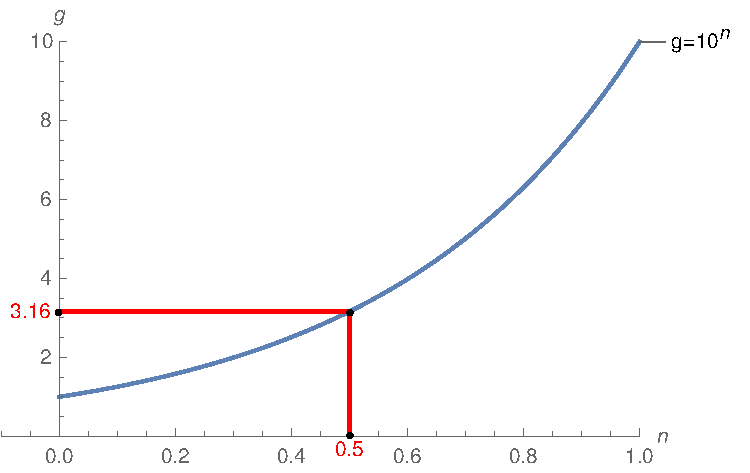
\includegraphics[width=0.7\linewidth]{figure/esponenziale.pdf}%
    \caption{Andamento dell'esponenziale $10^n$.}
    \label{fig:esponenziale}
\end{figure}

Il valore di $g$ equidistante (inteso in questo caso come rapporto tra misure) tanto da $1$ quanto da $10$ è dato dalla proporzione:
%%
\[
 \frac{g_{eq}}{1} = \frac{10}{g_{eq}}
\]
%%
dove co $g_{eq}$ si è indicata l'equidistanza cercata. Esplicitando si trova:
%%
\[
 g_{eq} = \sqrt{10} = 3,16227
\]

Il valore di $n$ corrispondente a $g_{eq}=3,16227$ si trova passando ai logaritmi:
%%
\[\begin{WithArrows}
 g_{eq} = 10^{n_{eq}}& \segue 3,16227 = 10^{n_{eq}} \segue \log(3,16227) = \log(10^{n_{eq}})\Arrow{}\\
			& \log(3,16227) = n_{eq}\,*\,\log(10) \segue n_{eq} = \dfrac{\log(3,16227)}{\log(10)} = 0,5
\end{WithArrows}\]
%%
valore che viene assunto come punto di separazione per stabilire l'ordine di grandezza di un numero.

Detto quindi $g=m*10^n$ un numero in forma esponenziale, si assumerà quale ordine di grandezza:
%%
\begin{equation}
 O_{(g)} = \begin{cases}
             10^n     & \text{per: }\, 1 < m \leq \sqrt{10} \\
             10^{n+1} & \text{per: }\, \sqrt{10} < m < 10
           \end{cases}\label{eq:odg_1}
\end{equation}

In modo analogo l'ordine di grandezza può essere valutato scegliendo quella potenza di $10$ tale che:
%%
\begin{equation}
 \frac{\sqrt{10}}{10} \leq m < \sqrt{10}\label{eq:odg_2}
\end{equation}
%%
o anche:
%%
\begin{equation}
 O_{(g)} = \begin{cases}
             10^n     & \text{se: }\, m \leq \sqrt{10} \\
             10^{n+1} & \text{se: }\, m > \sqrt{10}
           \end{cases}\label{eq:odg_3}
\end{equation}

\begin{example}{}
{Si confronti il raggio medio dell'atomo di idrogeno pari a $5,29*10^{-11}\meter$ con quello del raggio medio del suo nucleo pari a $1,2*10^{-15}\meter$}
        %%
{%
Utilizzando quanto previsto nei casi definiti nel sistema (\ref{eq:odg_1}) si trova:
%%
\begin{itemize}
 \item $O_{g1}$ di $5,29*10^{-11}\meter$: essendo $\sqrt{10}<m=5,29<10$ si trova che 
								$O_{g1}=10^{-11+1}=10^{-10}$;
 %%
 \item $O_{g2}$ di $1,2*10^{-15}\meter$: essendo $1<m=1,2<\sqrt{10}$ si trova che 
								$O_{g2}=10^{-15}$;
\end{itemize}

Utilizzando invece le condizioni della (\ref{eq:odg_2}) si ha:
%%
\begin{itemize}
 \item $O_{g1}$ di $5,29*10^{-11}\meter$: deve essere $\frac{\sqrt{10}}{10} \leq m < \sqrt{10}$ essendo $m=5,29>\sqrt{10}$, si moltiplica e si divide il raggio dell'atomo di idrogeno per $10$ in modo da far rientrare la mantissa entro i limiti stabiliti:
 \[ 5,29*10^{-11}\frac{10}{10} = 0,529*10^{-10} \]
 Segue quindi:
 \[
 \frac{\sqrt{10}}{10} \leq m=0,529 < \sqrt{10} \quad\text{segue quindi:}\quad O_{g1}=10^{-10}\]
 %%
 \item $O_{g2}$ di $1,2*10^{-15}\meter$: essendo $\frac{\sqrt{10}}{10} \leq m=1,29 < \sqrt{10}$ segue che $O_{g2}=10^{-15}$. 
\end{itemize}

Per le condizioni espresse nel sistema (\ref{eq:odg_3}) si arriva velocemente a stabilire gli ordini di grandezza già definiti. Il confronto tra i due raggi è quindi:
%%
\[
 \frac{O_{g1}}{O_{g2}} = \frac{10^{-10}}{10^{-15}} = 
																			10^{-10}*10^{15} = 10^{-10+15} = 10^5 = 100.000
\]

Il raggio dell'atomo di idrogeno ha quindi un raggio che è $100.000$ volte più grande di quello del suo nucleo}
\end{example}


				\section{Cifre significative e arrotondamenti}

Determinare il risultato di un calcolo derivato da una serie di misure, significa anche stabilire il numero di cifre con le quali deve essere registrato. È infatti privo di senso scorretto esprimere un calcolo con un numero arbitrario di cifre senza tener conto dell'\hlightit{indeterminazione}, \hlightit{incertezza} o \hlightit{errore} (per esempio quello \hlightit{assoluto}) correlato a quelle stesse misure.

Analoghe considerazioni vanno fatte per gli errori per i quali un numero eccessivo di cifre è privo di senso a causa della natura \textit{statistica} e \textit{probabilistica} di cui gli errori sono affetti.

Va anche tenuto presente che non solo è errato l'uso eccessivo di cifre, ma lo è anche ridurle pericolosamente senza tener conto delle approssimazioni e del contenuto informativo necessario.

Sia per esempio l'incertezza relativa alla misura di un tempo pari a:
%%
\[
 \eass[t] = 0,02\second
\]
%%
dove $\eass[t]$ è espresso in centesimi di secondo.

Ebbene, trascrivere tempi determinati da calcoli successivi come:
%%
\[
 t_1 = 5,1\second \quad\text{oppure}\quad t_2 = 5,12357\second
\]
%%
è scorretto perché nel primo caso non viene indicata la cifra corrispondente ai centesimi di secondo con la conseguente perdita di contenuto informativo, mentre nel secondo vengono date cifre che vanno ben oltre quelle stabilite da $\eass[t]$.

I dati, specie se frutto di calcoli, vanno quindi espressi con un numero di cifre corrispondente alla precisione:
%%
						\begin{fancyquote}
							\emph{per convenzione si scrive l'errore con un numero di cifre significative non maggiori di due, mentre la misura dovrà essere scritta con un numero di cifre tale, che quella più a destra occupi il medesimo posto, rispetto alla virgola, di quella che nell'errore occupa il posto più a destra}.
						\end{fancyquote}

È quindi corretto scrivere:
%%
\[
      t_1 = (5,12 \pm 0,02)\second \quad\text{oppure}\quad R = (54,1 \pm 0,1)\ohm
\]
%%
mentre per esempio è \textbf{errato} scrivere:
%%
\[
      U = (12,30 \pm 0,1)\volt
\]
%%
perché la cifra più a destra del dato --lo ``$\,0\,$''-- definisce i centesimi di volt, mentre l'``$\,1\,$'' dell'incertezza solo le decine.

L'errore consiste nel non aver considerato lo ``$\,0\,$'' del dato una cifra, quale invece è, \textit{significativa}. Scrivere infatti:
%%
\[
   12,30\volt \quad \text{e} \quad 12,3\volt
\]
%%
dà ai numeri un significato totalmente diverso perché nel primo caso si assume, per esempio, un errore assoluto pari a $0,01\volt$, mentre nel secondo uno uguale a $0,1\volt$. Occorre quindi stabilire e definire cosa si debba intendere per \hlightit{cifra significativa}.

In termini generali si può dire che sono \textit{cifre significative quelle i cui valori sono certi, più la prima cifra il cui valore è incerto}. In particolare si può affermare che:
%%
				\begin{fancyquote}
				  \emph{le cifre significative sono il numero minimo di cifre con cui è possibile esprimere il valore di una grandezza, senza che vi sia un aumento dell'incertezza e, quindi, perdita dell'accuratezza}.
				\end{fancyquote}

In pratica il numero di \textit{cifre significative si conta partendo dalla prima cifra incerta più a destra, fino ad arrivare a quella più significativa posta più a sinistra e diversa da zero}. Alcuni esempi di numero di cifre significative sono dati nella tabella~\ref{tab:cifresignificative} dove viene messa in evidenza l'importanza degli zeri.

\begin{table}[htp!]
\begin{center}
\caption{Numero di cifre significative.}\label{tab:cifresignificative}
\cifresignificative
\end{center}
\end{table}

Per stabilire quali cifre significative si adotteranno i seguenti criteri:
%%
\begin{itemize}
 \item gli zeri compresi tra due cifre significative \textbf{non nulle} vanno considerati. Esempio:\par
  {\centering $21007$ ha \textbf{5} cifre significative, $5,09$ ha \textbf{3} cifre significative\par}
 %%
 \item gli zeri più a sinistra e oltre l'ultima cifra \textbf{diversa da zero} non vanno considerati. Esempio:\par
 {\centering $0,03$ e $0,005$ hanno entrambi \textbf{una} sola cifra significativa\par}
 %%
 \item gli zeri più a destra che sono dopo la virgola e oltre l'ultima cifra \textbf{non nulla}, sono significativi: Esempio:\par
 {\centering $2,0$ ha \textbf{2} cifre significative, $0,0100$ ha \textbf{3} cifre significative\par}
 %%
 \item gli zeri possono essere \textbf{non necessariamente significativi} se sono posti alla fine di un \textbf{numero intero}. Sia per esempio la misura $2100\meter$. Si intende $(2100\pm 1,0)\meter$ oppure $(2100\pm 1)\meter$. Per eliminare l'ambiguità deve essere scritto secondo la notazione scientifica:
 \begin{itemize}
  \item $2,100*10^3$ se si vuol dare significato alla cifra delle \textit{unità}. I questo caso il numero ha \textbf{4} cifre decimali;
 %%
  \item $2,10*10^3$ se si vuol dare significato alla cifra delle \textit{decine}. Il numero ha \textbf{3} cifre decimali; 
 %%
  \item $2,1*10^3$ se si vuol dare significato alla cifra delle \textit{centinaia}. Il numero ha \textbf{2} cifre decimali. 
 \end{itemize}
\end{itemize}




















